% ------------------------------------------------------------------------
%                             Capítulo 2
% ------------------------------------------------------------------------
\chapter{Algoritmos y herramientas}
En este capítulo se describen los algoritmos y herramientas utilizados para la realización de este \ac{TFG}; así como los principales motivos para su elección.

\section{Matlab}
Para el desarrollo del algoritmo se necesita un entorno de programación que aporte las funciones necesarias de tratamiento de imagen y que, al mismo tiempo, facilite la manipulación y depuración de código. Por ello se ha elegido el entorno Matlab.\\

Dicho entorno ha sido elegido de acuerdo a las siguientes razones:
\begin{itemize}
\item Experiencia previa en el uso del entorno Matlab en distintas asignaturas cursadas durante la carrera.
\item Facilita el tratamiento digital de imagen gracias al gran número de funciones disponibles.
\item Permite la representación de imágenes como matrices, lo que simplifica su tratamiento.
\item Existencia de abundante documentación y una gran comunidad de usuarios.
\end{itemize}

\section{OpenCV 4.8}
Para poder ejecutarlo en la placa Raspberry Pi, necesitamos portar nuestro código desarrollado en Matlab a C++. Dicha tarea requiere el uso de funciones de tratamiento digital de imagen. Para ello, recurrimos a la librería gráfica OpenCV.\\

Entre las razones para la elección de esta librería en particular destacan:
\begin{itemize}
\item Soporte para múltiples plataformas y sistemas operativos, siendo particularmente interesante el soporte para Raspberry Pi y Linux.
\item Incluye todas las funciones necesarias para portar el algoritmo.
\item Es software libre, por lo que está disponible de forma completamente abierta sin licencias privativas.
\item Existencia de abundante documentación y una gran comunidad de usuarios.
\end{itemize}

\section{Algoritmo de detección de contornos}\label{canny}
La detención de contornos es un proceso mediante el cual, a partir de una imagen en escala de grises, obtenemos las zonas dónde se producen fuertes discontinuidades. Dichas discontinuidades generalmente coinciden con los bordes de los objetos retratados por la imagen.

Este procedimiento resulta útil para un gran número de aplicaciones, ya que un mapa de contornos contiene parte significativa de la información almacenada en la imagen, pero con una complejidad mucho menor. \cite{IEEEedge} Un ejemplo de mapa de contornos puede verse en la \reff{contornos}.\\

\begin{figure}[!h]
\centering \subfigure[Original.]{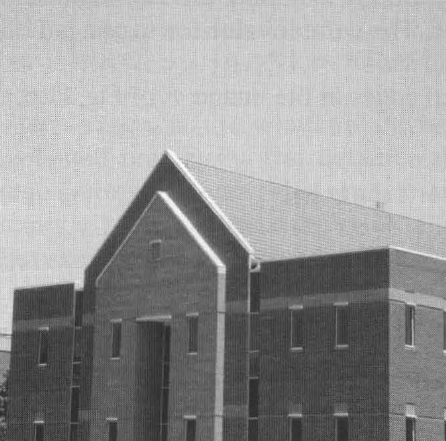
\includegraphics[width=6cm]{Ejem_Cont_Org.png}}
\subfigure[Mapa de contornos.]{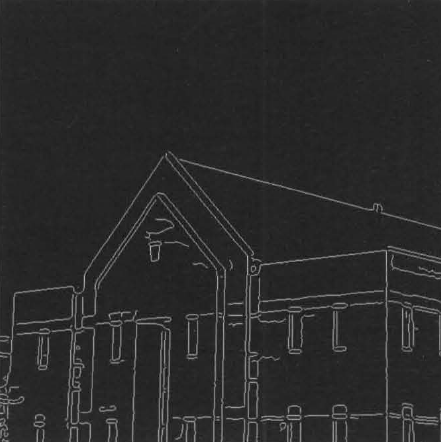
\includegraphics[width=6cm]{Ejem_Cont_Result.png}}
\caption{\small{Efecto del escalado sobre la imagen. Fuente:} \cite{ImgProcessMat}} \label{contornos}
\end{figure}

La figura (a) representa la imagen original en escala de grises, mientras que la figura (b) representa el mapa de contornos obtenido. Como puede apreciarse, la imagen (b) tiene una complejidad menor, ya que sólo contiene información acerca de los bordes de los objetos representados. 

Esta información resulta suficiente para numerosas aplicaciones que traten de localizar objetos dentro de una imagen, como la aplicación \ac{ALPR} que nos ocupa.\\

La idea básica para buscar un mapa de contornos es encontrar las partes de la imagen donde la intensidad cambia rápidamente usando estos dos criterios:

\begin{enumerate}
\item Encontrar las zonas donde la primera derivada es mayor que un determinado umbral.
\item Encontrar las zonas donde la segunda derivada presenta un cruce por cero.
\end{enumerate}


En tratamiento de imagen la primera derivada es el gradiente de una función de dos dimensiones, cuya expresión viene dada por la ecuación:

\begin{equation}
\boldsymbol{\nabla f}= \left[ \begin{array}{c} G_{x} \\ G_{y}  \end{array} \right] =  \left[ \begin{array}{c} \frac{\partial f}{\partial x} \\ \frac{\partial f}{\partial y}  \end{array} \right]
 \label{ecuacion1}
\end{equation}

El algoritmo trabaja con la magnitud de este vector calculada de la siguiente forma:

\begin{equation}
\nabla f=mag( \boldsymbol{\nabla f})=\sqrt{[G_{x}^{2}+G_{x}^{2}]}
\end{equation}

En cuanto a la derivada de segundo orden, normalmente es calculada usando el Laplaciano, como muestra la ecuación:

\begin{equation}
\nabla^{2}f(x,y)=\frac{\partial ^{2} f(x,y)}{\partial x^{2}} + \frac{\partial ^{2} f(x,y)}{\partial y^{2}}
\end{equation}





Existen multitud de algoritmos para detectar los contornos en una imagen. En este \ac{TFG} se han realizado pruebas con dos de los más conocidos: el algoritmo de Canny y el algoritmo de Sobel.

\subsection{Algoritmo de Sobel}
La principal característica del algoritmo de Sobel es que calcula la primera derivada  mediante una aproximación basada en las diferencias entre filas y columnas de los píxeles vecinos en un área de 3X3 como muestra la Ecuación \refe{ecuacion1} y la  \reff{VecinosSobel}.

\begin{figure}[!h]
\centering
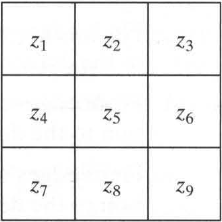
\includegraphics[width=3cm]{VecinosSovel.png}
\caption{\small{Vecinos en el algoritmo de Sobel. Fuente:}\cite{ImgProcessMat}}
\label{VecinosSobel}
\end{figure}

\begin{equation}
g= \sqrt{G_{x}^{2}+G_{x}^{2}}
= \sqrt{[(z_{7} + 2z_{8} + z_{9})-(z_{1} + 2z_{2} + z_{3})]^{2} + (z_{3} + 2z_{6} + z_{9})-(z_{1} + 2z_{4} + z_{7})]^{2} }
\label{ecuacion1}
\end{equation}

Por tanto, decimos que un píxel en una localización determinada (x,y) pertenece a un contorno si g $\geq$ T, siendo T un umbral determinado previamente. \\

En caso de no especificarse el valor del parámetro, el algoritmo lo calcula por sí mismo; siendo ademas posible indicarle una dirección preferente (horizontal o vertical) para buscar los contornos.\\

Se eligió este algoritmo en primer lugar debido a su facilidad de uso, ya que no es necesario ajustar ningún parámetro. El resultado, sin especificar ningún umbral y marcando como dirección preferente la horizontal, se muestra en la \reff{EjemploSobel}.

\begin{figure}[!h]
\centering
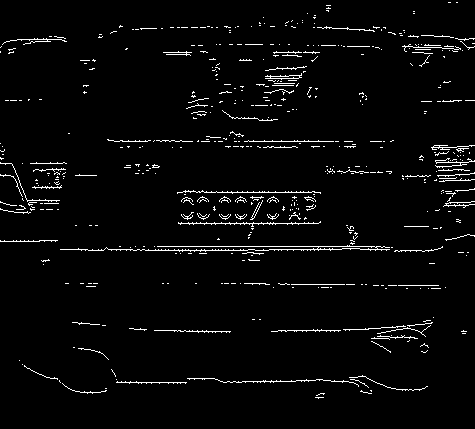
\includegraphics[width=6cm]{EjemploSobel.png}
\caption{\small{Resultado de la detección de ejes con el algoritmo de Sobel.}}
\label{EjemploSobel}
\end{figure}

Como se puede observar en la imagen, el resultado no cumple con las necesidades de la aplicación: aparece mucho ruido en la imagen y las líneas contienen numerosas discontinuidades. 

Para resolver el problema tratado en este \ac{TFG} se necesita un mapa de contornos más simple. Es decir: sólo es necesario que aparezcan los contornos más representativos, que deben estar bien definidos y sin discontinuidades.

\subsection{Algoritmo de Canny}
El algoritmo detector de Canny consta de cuatro pasos:

\begin{enumerate}
\item El ruido de la imagen se reduce mediante el uso de un filtro gaussiano de  desviación típica $\sigma$.

\item Se calcula la primera derivada de la imagen empleando el mismo método que el algoritmo de Sobel.

\item Aplica dos umbrales T1 y T2, siendo T1$<$T2, a la primera derivada calculada anteriormente. Los píxeles para los que el valor es mayor que T2 son llamados píxeles fuertes, mientras que aquellos con un valor entre T1 y T2 son llamados píxeles débiles. A los demás se les fija su valor a 0. Este proceso se conoce como \emph{nonmaximal suppression.}

%\item Los puntos calculados en el apartado anterior dan lugar a picos en el gradiente de la imagen. El algoritmo busca la cima de esos picos y fija a cero todos los píxeles que no pertenecen a ella, conociéndose este proceso como \emph{nonmaximal suppression.} Los píxeles de la cima se determinan mediante dos umbrales T1 y T2, siendo T1$<$T2, los píxeles con un gradiente mayor que T2 son llamados píxeles fuertes y aquellos con un valor entre T1 y T2 son llamados píxeles débiles.

\item Finalmente, el algoritmo forma el contorno incorporando a los píxeles fuertes los píxeles débiles que se encuentren a una distancia de ocho píxeles o menos. 
\end{enumerate}

Se han realizado pruebas con este algoritmo por ser el más potente de los algoritmos de detección de contornos, pero, al contrario que con el algoritmo de Sobel, debemos ajustar los parámetros de la desviación estándar  y los umbrales. El resultado, tras una correcta calibración, se muestra en la \reff{EjemploCanny}\\

\begin{figure}[!h]
\centering
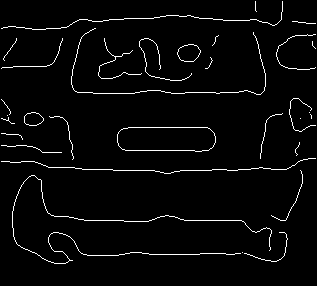
\includegraphics[width=6cm]{EjemploCanny.png}
\caption{\small{Resultado de la detección de ejes con el algoritmo de Canny.}}
\label{EjemploCanny}
\end{figure}

Los resultados son significativamente mejores que los obtenidos con el algoritmo de Sobel. En esta ocasión sólo aparecen los contornos más significativos de la imagen, y las líneas están perfectamente definidas. Por tanto, éste es el algoritmo elegido finalmente para llevar a cabo el detector de matrículas.\\

Para más información sobre los algoritmos de detección de contornos consultar \cite{ImgProcess}.

\section{Transformada de Hough}\label{hough}
Dada una imagen binaria, si queremos encontrar subconjuntos de píxeles que formen líneas rectas, una posible solución es encontrar primero todas las líneas formadas por cada par de píxeles para, posteriormente, buscar todos los píxeles que se encuentren próximos a cada una de la líneas.

El problema de esta solución es que es necesario encontrar $n(n-1)/2 \simeq n^{2}$ líneas así como realizar $n(n(n-1))/2 \simeq n^{3}$ comparaciones entre los n píxeles y todas las líneas. Esta solución resulta computacionalmente irrealizable en cualquier aplicación, excepto en los ejemplos más triviales.\\

Para realizar una aproximación al problema de la detección de líneas rectas que el sistema pueda soportar empleamos la transformada de Hough.\\

Sea un punto $(x_{i},y_{i})$. Las infinitas líneas que pasan a través de él satisfacen la ecuación $y_{i}=ax_{i}+b$. Si se reorganiza la ecuación escribiéndola de la forma $b=-ax_{i}+y_{i}$ y se considera el plano ab\footnote{Plano ortonormal con la variable $b$ en el eje de abscisas y la variable $a$ en el eje de ordenadas}, el punto $(x_{i},y_{i})$ determina de forma inequívoca una recta. Sea otro punto $(x_{j},y_{j})$. Éste determinará otra recta en el plano ab. Dicha recta se cortará con la anterior en el punto $(a' , b')$, siendo $a'$ la pendiente de la recta que determinan los dos puntos en el plano $xy$, y $b'$ el corte de dicha recta con $x=0$. Esta idea queda ilustrada en la  \reff{planoab}. \\

\begin{figure}[!h]
\centering
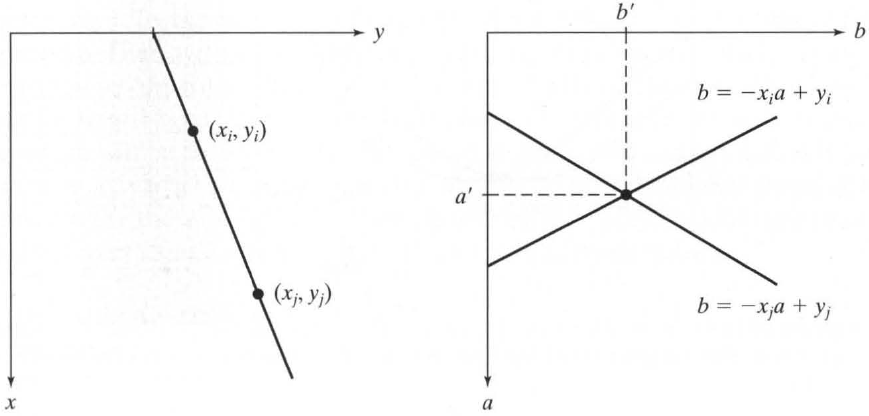
\includegraphics[width=12cm]{planoab.png}
\caption{\small{Relación entre el plano $xy$ y el plano $ab$. Fuente:\cite{ImgProcessMat}}}
\label{planoab}
\end{figure}

De esta forma, usando el plano $ab$ podrían calcularse todas las líneas correspondientes a cada píxel de la imagen; siendo posible determinar las principales líneas rectas simplemente buscando aquellos puntos en el plano $ab$ donde intersecten un gran número de líneas.\\

Una dificultad que presenta esta técnica es que cuando $a$ tiende a infinito, las rectas tienden a ser verticales. Por este motivo, se realiza un cambio a coordenadas esféricas quedando la ecuación, de la recta de la siguiente forma:
\begin{equation}
x \cos{\theta} + y \sin{\theta} = \rho
\end{equation}

Con ésta representación, el plano $ab$ pasa a ser el plano $\theta\rho$; tal y cómo muestra la \reff{planoabesf}. \\

\begin{figure}[!h]
\centering
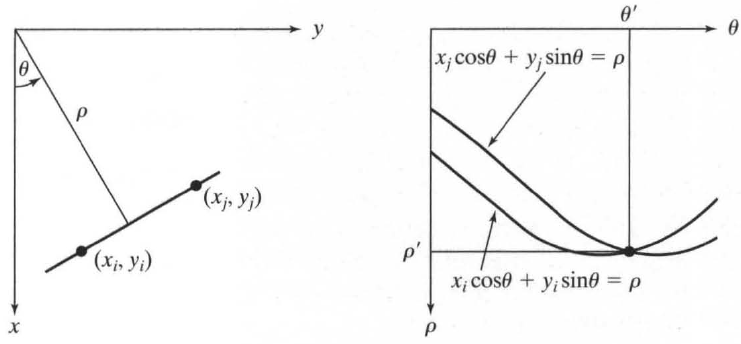
\includegraphics[width=12cm]{planoabesfericas.png}
\caption{\small{Relación entre el plano $xy$ y el plano $ab$ en esféricas. Fuente:\cite{ImgProcessMat}}}
\label{planoabesf}
\end{figure}


Para más información sobre la detección de líneas rectas mediante transformada de Hough consultar \cite{ImgProcess}.